% REV00 Tue 20 Jul 2021 08:12:01 WIB
% START Tue 20 Jul 2021 08:12:01 WIB

\chapter{Empatbelas}

% 11
\begin{figure}[htbp]
% h: here, where the figure appears in the text (use can always just use [h] )
% t: top,  top of the current page.
% b: bottom of the current page.
% p: page, top of the next available float space (sometimes end up being the end of the document).
\centerline{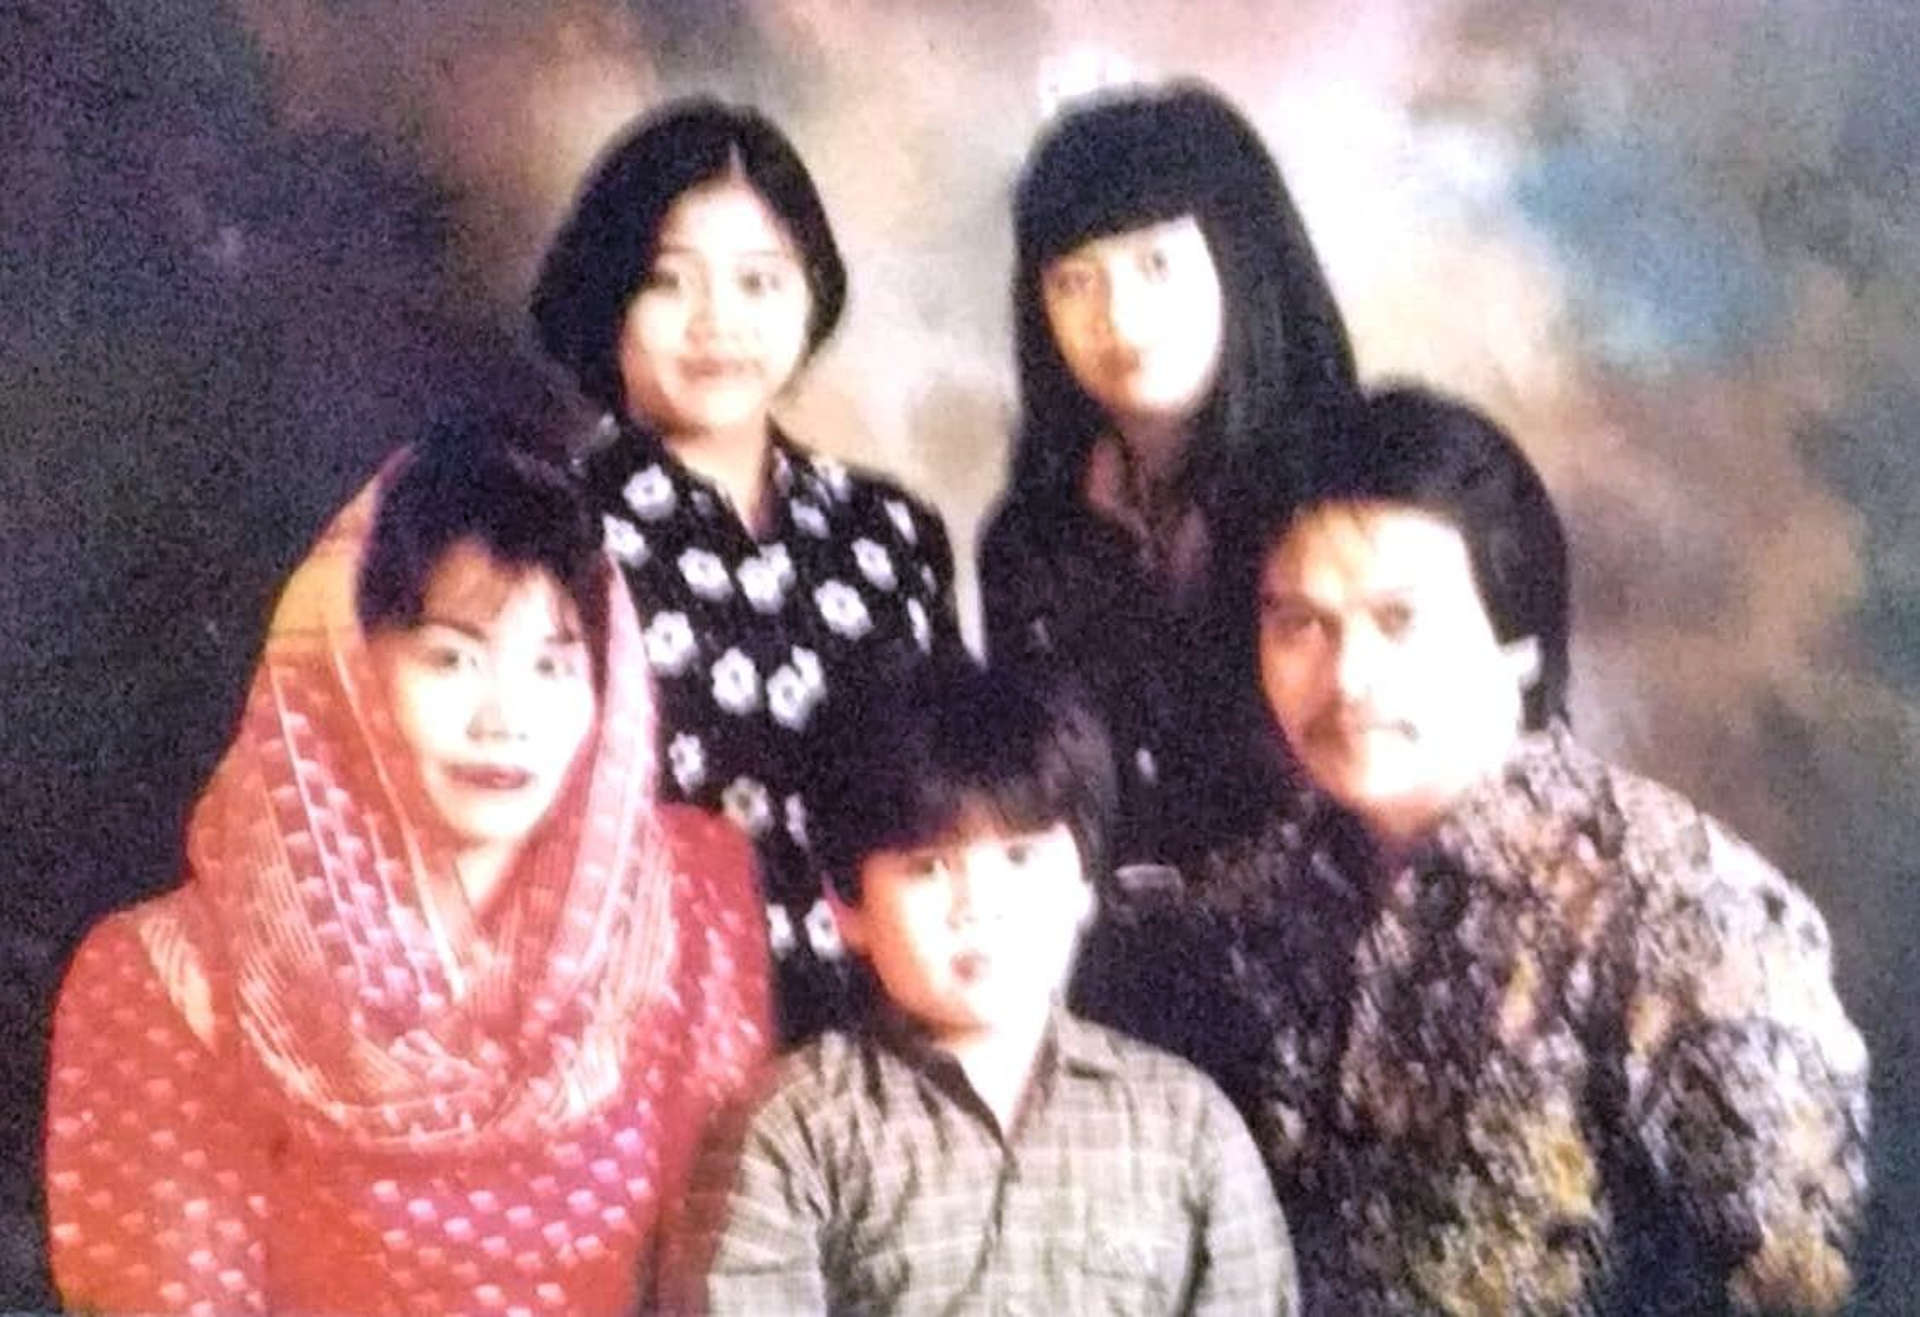
\includegraphics[scale=1.0]{01-14-01}}
\caption{"Album Keluarga Sekembali dari Nigeria" Sumber: Koleksi Kelvy Safira dan Fitria Clara Zora.}
\label{01-14-01}
\end{figure}
%

Bukannya ke Argentina, Satiri malah naik jabatan dari Senior Field Engineer (atasannya tukang di lapangan) menjadi Engineer in Charge (mandor) di Prabumulih, Palembang.

Enak banyak duren dan duku. Kliennya juga Cuma satu: Pertamina. Di sini untuk pertama kali dia belajar bagaimana kata 'cingcai' bekerja: Dua tambah dua boleh berapa saja, isi sendiri, sekenyangnya dan 'sepantasnya'

Dengan jabatan mandor, dia mulai diminta menjadi instruktur. Di ruang kelas dan praktikum di fasilitas Schlumberger, Medan. Ini peran pertamanya menjadi guru.

Baginya menarik juga melihat anak-anak antusias belajar. Walaupun ya biasalah jahil-nya tidak berkurang. Dia sering mengerjai mereka supaya kelas menjadi segar dan peserta tahu betul masalah di lapangan.

Dia mulai bosan, dan isengnya kambuh. Dia minta jabatannya naik lagi. Dikasih juga.

Tiga tahun di Prabumulih, dia dinaikan menjadi Field Service Manager (atasannya mandor) di Jambi. Kali ini kliennya lebih banyak: Asamera, Santa Fe, dan Pertamina. Gaji naik, tanggung jawab tambah banyak. Pekerjaan lobby tak ada henti.

Anak-anaknya pun semakin besar, butuh sekolah dan mengenal keluarga.

“Kita harus balik ke Jakarta,” itu keputusan yang dia sampaikan ke istrinya.

Belum tiga tahun di Jambi, pindahlah dia ke Schlumberger Jakarta. Jabatan masih sama, kliennya kalau ini beda: BP dan ARCO. Di sanapun ia hanya bertahan sembilan bulan.

Kebosanan sungguh musuh yang sukar dikalahkan. Dia membuthkan sesuatu yang berbeda untuk pikirannya, bukan lagi untuk kantungnya.

“Gua mau berenti kerja. Bosen,” katanya kepada istrinya. Anda tahulah budaya ‘orang lapangan’ yang penuh godaan, cobaan, dan gangguan. Apa ada yang 100% berhasil mengatasinya?

“Ya terserah abang, kalau itu yang abang mau…” Istrinya yakin uang bukan masalah.

Benar saja. Tengah Desember 1996, Schlumberger melepaskan dirinya dengan dua kopor uang pensiun. Tetapi ekornya tetap dipegangi.

Januari 1997 dia mulia kuliah lagi. Sesuatu yang lumayan rada berbeda.

“Sekolah yang nggak usah terlalu serius saja Ren, sambil nemenin anak-anak belajar” katanya suatu ketika kepadaku.

Sesungguhnya sekolahnya itu lumayan ada nama, program MBA International Management di IPMI Jakarta, yang bekerjasama dengan Monash University, Australia.

Walaupun tidak serius, dengan berbagai pengalamannya di lapangan dia lulus dengan predikat cum laude dalam setahun saja. Ternyata sekolah ini juga sungguh candaan belaka baginya.

Dua bulan sebelum wisuda dia sudah diminta Schlumberger GeoQuest Jakarta untuk bergabung. Kali ini dia diminta untuk menjadi Sales Manager (tukang jualan). Kalau Satiri remaja asongannya kembang, kini asongannya software manajemen data. Kliennya Pertamina, BP MIGAS, VICO, LASMO, TFE dll. Serba keren, dan harus pakai jas. Sesuatu yang mulai ia biasakan.

“Harga software enggak ada patokannya, Ren. Enak, suka-suka,” katanya kepadaku. Waktu itu Satiri dengan baby benz boxernya mampir ke kantorku, kantor pusat urusan tenaga atom di bilangan Mampang. Parkir mobilnya berdampingan dengan mobil Dirjen yang sederhana. Kontras.

Dalam obrolan itu Satiri kemudian menjelaskan beberapa pelajaran yang menurutnya berharga sebagai tukang jualan. Antara lain:

Menemui klien atau calon klien: “Kita lebih baik nunggu satu jam, dari pada telat 5 menit.”

Menemui pejabat: “Kita serius saja mendengarkan ocehannya. Tanggapi positif kalau memang dia nampak minta ditanggapi. Nanti kalau dia sudah capek dia juga nanya kita mau apa. Nah, itu artinya kupingnya sudah siap dia buka buat dagangan kita…”

Menilai perusahaan: “Kalau gua digaji 100, itu artinya untung perusahaan minimal 1000…”

Begitulah Satiri berdagang secara prestisius, dan elit. Sebab, tukang jualan GeoQuest juga hanya dua orang saja, hemat dan jelas targetnya. Tukang jualan yang satunya lagi adalah Bang SAS, Fisika ’76, seniornya.

(Fisika itu sesungguhnya bisa jadi apa saja. Jadi menteri kesehatan juga bisa kan… Elon Musk juga anak Fisika. Buat anak Fisika jangan GR ya, anak SMA juga bisa jadi menteri!)

“Sebagai pegawai Schlumberger internasional, gua di Jakarta ini dikasih tunjangan perumahan 3000\$ sebulan. Kartu kredit tanpa batas dan semua rekening apapun dibayar perusahaan,” ujarnya merendah, eeh… “Dan, itu belum termasuk gaji…”

“Tapi kartu kreditnya enggak pernah gua pake buat keluarga…” Rupanya dia masih teringat kuitansi tukang sayur dan cap Himafi. Hahaha… Baguslah.

Jadi kartu kreditnya dipakai apa?

Itu untuk beli tiket pp ke Huston, LA, Las Vegas, atau mana saja, biaya hotel, makan-makan, belanja-belanja buat para boss. Pengambil keputusan teknis maupun strategis di instansi yang berhubungan dengan kebijakan minyak. Apa aja boleh, asal tidak terbukti melawan hukum, dan dagangan laku.

Ini jugalah yang menentukan harga BBM dan besarnya subsidi. Hmmm….

Siapa yang ditraktir bisnis itu? Sebagian besar ya teman-temannya kuliahnya jugalah. Hayo siapa yang ikut baca cerita ini dan pernah diongkosi Satiri? Hahahahah…

***

Di puncak gunung tertinggi, anda tidak lagi menghadapi siapa-siapa. Anda hanya akan menghadapi diri anda sendiri. Mungkin begitulah salah satu yang ingin dikatakan Fariduddin Attar dalam “Musyawarah Burung” (Mantiqut Thair).

Aku kira selain menghadapi dirinya, dia juga bertatapan dengan kebosanan.

Tetapi lumayanlah dia bisa bertahan empat tahun di GeoQuest. Apa lagi sekarang?

Terdengar lengkingan Barbra Streissand dan Donna Summer melantunkan “No More Tears” dengan nada-nada tinggi:

“Enough is enouh. I can’t go on. I can’t go on…”

Baiklah, mari kita menghadap Boss-nya yang bule. Kata Satiri, di level bossnya ini tidak ada orang selain yang bule.

“Boss saya mau berhenti,” katanya tanpa basa-basi.

“Apalagi sekarang, lu mau naik gaji berapa?” juga tanpa basa-basi.

“I want to sit on your chair.”

“Fcuk you!” kata boss-nya sambil menandatangani surat pengunduran diri Satiri. Mereka berdua bersalaman, berpelukan, tertawa bersama, dan bahkan saling mendoakan sebelum berpisah.
.
.
***

“Bosen Ren, lihat kelakuan mereka,” katanya kepadaku.

“Di industri minyak ini kan banyak banget bule-bule. Emangnya mereka juga ikut kongkalikong…”

“Yaah, Reno, lu polos banget. Semua bule itu awalnya memang jujur. Enggak bakal lebih dari enam bulan, gua jamin, mereka mulai mumet. Terus ikutan deh sama kita-kita…”

Dia kemudian bercerita pernah dilibatkan Pemerintah untuk memperbaiki kebijakan energi. Dengan polosnya ia menceritakan berbagai hal strategis yang seharusnya diambil Pemerintah dan berbagai efisiensi yang dapat dilakukan.

“Hahahah…” Aku terpingkal-pingkal mendengarnya. Kaget dia mendengar aku tertawa.

“Lah?”

“Yang polos itu elu Bang,” kataku.

“Koq bisa?”

“Mereka tuh para pejabat enggak bodoh. Mereka hanya mau ngecek, orang-orang pintar kayak ente itu tahu enggak skenario korupsi yang sedang mereka rencanakan…”

“Laah, suudzon dong…”

“Kan abang sendiri yang bilang bahwa minyak itu waktu diambil dari perut bumi warnanya hitam gelap. Bisnisnya begitu juga kali yah…”

Hahahah… Kami tertawa bersama sambil nyeruput kopi Kapal Api, kopi kebanggaan, di kantin kecil belakang Gedung B.

Itulah tawa kami bersama mengakhiri kariernya di minyak. Kata-kata ajaib masa kecilnya ‘elektronika, ‘minyak’, dan ‘Australia’ sudah terlaksana, walaupun ‘Rusia’ tentunya sudah diwakili sekurang-kurangnya oleh Nigeria, Prancis, Italia, Belanda dan Amerika.

Apalagi yang akan ia lakukan?
\\[10pt]

Sumber tulisan asli \url{https://www.facebook.com/reno.alamsyah.94/posts/10226600785191923}

